\subsection{Synthetische Daten}\label{sec:synthetic_data}

Die Erzeugung synthetischer Daten wurde im Jahre 2016 maßgeblich durch die Generative Adversarial Architektur, auch GAN genannt, beeinflusst \cite{P-86}. 
Bei dieser Architektur gibt es 2 gegensätzliche Neuronale Netzwerke, der Generator und der Diskriminator. 
Der Diskriminator lernt dabei, zwischen echten Daten und nicht echten Daten zu unterscheiden, die abwechselnd von dem echten Datensatz und dem Generator kommen.
Im Gegensatz dazu, versucht der Generator, Daten zu erzeugen, die den Diskriminator täuschen. 
Der Diskriminator kann dabei 2 Verlustfunktionen haben, einmal für sich selber und einmal für den Generator.
Die Verlustfunktion des Generators kann dabei durch den Generator backpropagiert werden, wodurch dieser immer realistischere Daten generiert.
Im besten Falle, erzeugt der Generator nach dem Training Daten, die so echt wirken, dass der Diskriminator diese nicht mehr unterscheiden kann.
Folglich erzeugt der Generator synthetische Daten, die latente Strukturen der originalen Daten enthalten.
Abbildung \ref{fig:gan} die bereits beschriebene Architektur.

\begin{figure}[!htb]
    \centering
    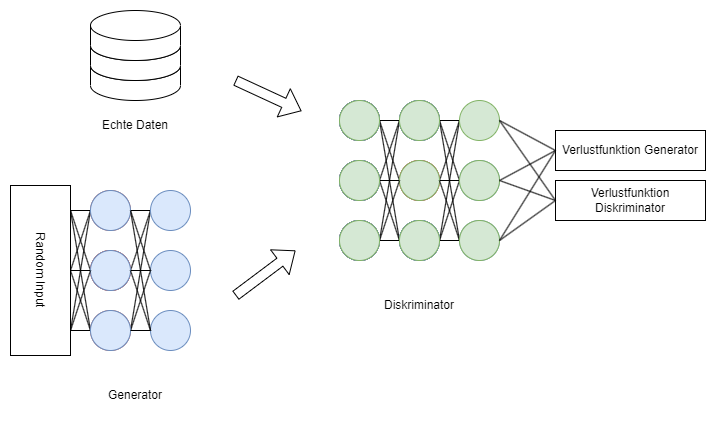
\includegraphics[width=14cm]{figures/gan}
    \caption{Generative Adversarial Network nach \cite{P-86}}
    \label{fig:gan}
\end{figure} 

Die Erzeugung von Daten mittels GANs kann nicht nur für Angriffe genutzt werden (siehe Kapitel \ref{sec:angriffe}), sondern auch für das Training von Neuronalen Netzen.
Eine Erweiterung der GANs ist das sogenannte Wasserstein GAN oder auch kurz WGAN \cite{P-92}. 
Standardmäßig kann bei GANs der Fall auftreten, dass die erzeugten Daten nicht jeden Teil einer Verteilung abbilden, sondern nur einen (z. B. den Häufigsten).
Um dieses Problem zu mindern, wird beim WGAN die Verlustfunktion des Diskriminators verändert. 
Anstatt einer binären Klassifikation (echt oder unecht), wird die Wasserstein-Distanz genutzt, welche angibt, wie viel Arbeit benötigt wird, um eine Verteilung in eine andere Verteilung zu transformieren. 
Die Wasserstein-Distanz gleicht der Earth Mover Distanz aus Kapitel \ref{sec:anonymisierung}.
Diese Metrik als Verlustfunktion ist jedoch nur nützlich, wenn nicht mit einzelnen Datenpunkten gearbeitet, sondern jeweils mit Batches trainiert wird.
Der Austausch der Verlustfunktion sorgt dafür, dass der der Generator Daten aus der ganzen Verteilung der Daten nachstellen muss und nicht nur aus einem Teil dieser.


Xie et al. \cite{P-70} stellen eine besondere Form des GANs vor, das sogenannte Differentially Private Generative Adversarial Network oder kurz DPGAN.
Dieses DPGAN nutzt als Basis das WGAN, fügt jedoch bei Berechnung der Verlustfunktion (Wasserstein-Distanz) Rauschen mittels des Gauß-Mechanismus aus Kapitel \ref{sec:dp} hinzu.
Durch die Eigenschaft, dass Differential Privacy resistent gegenüber Nachbearbeitung ist, kann auch garantiert werden, dass die Gradienten, die im Generator ankommen, mittels Differential Privacy geschützt sind.
Die Autoren können zeigen, dass es möglich ist, Bilder des MNIST Datensatzes zu erzeugen.
Abbildung \ref{fig:dpgan} zeigt diese Erzeugung mit unterschiedlichen $\epsilon$ Werten.
Es ist zu sehen, dass bei kleiner werdendem $\epsilon$, die Qualität der Bilder schlechter wird und auch mehr Daten der falschen Klasse erzeugt werden. 
Bei $\epsilon=9,6$ ist die Anzahl an Daten mit falschem Label größer, als die Anzahl der Daten mit richtigem Label.
Folglich ist die Wahl von $\epsilon$ entscheidend, wie gut die synthetischen Daten die Originaldaten wiedergeben.

\begin{figure}[!htb]
    \centering
    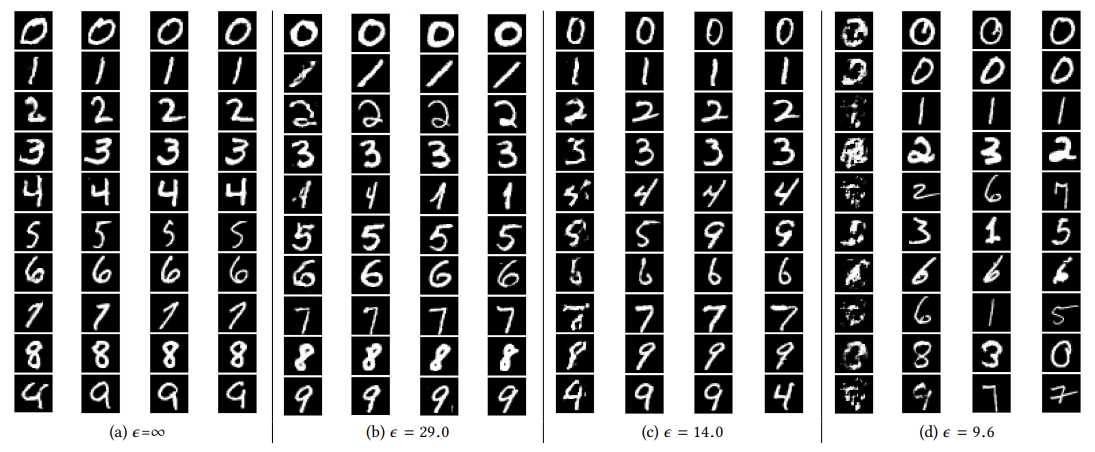
\includegraphics[width=15cm]{figures/dpgan}
    \caption{Syntehtischer MNIST Datensatz mittels DPGAN \cite{P-70}}
    \label{fig:dpgan}
\end{figure} 

Jordon et al. \cite{P-68} stellten eine alternative Form des GANs vor, welches ebenfalls synthetische Daten erzeugt. 
Dieses nutzt das Private Aggregation of Teachen Ensembles Framework, kurz PATE, welches in Kapitel \ref{sec:pate} im Detail beleuchtet wird.
Bei der PATE Architektur, werden die Daten in verschiedene Teildatensätze unterteilt. 
Verschiedene Modelle, die sogenannten Lehrer oder Teacher, lernen die Klassifikation jeweils an einem unterschiedlichen Teildatensatz.
Ein weiteres Modell, welches Schüler oder Student genannt wird, kann nun mittels des Exponential-Mechanismus aus \ref{fig:dp} aus den aggregierten Vorhersagen der Lehrer Modelle, eine Klasse vorhersagen.
Das PATE-GAN nutzt die PATE Architektur für den Diskriminator, welcher ein binärer Klassifikator ist.
Wie das DPGAN, nutzt auch das PATE-GAN die Resistenz gegenüber Nachbearbeitungen von Differential Privacy aus, um Differential Privacy auch für die synthetischen Daten zu garantieren.


Ein Algorithmus, welcher kein GAN zur Erzeugung künstlicher Daten nutzt, ist NIST-MST von McKenna et al. \cite{P-95}.
Mit NIST-MST gewannen McKenna et al. die \textit{Differential Privacy Synthetic Data Competition}, welche vom National Institute of Standards and Technology der USA ausgetragen wurde.
Neben NIST-MST, welcher auf den obigen Wettbewerb angepasst wurde, gibt es noch MST für generelle Anwendungsfälle.
MST besteht dabei aus 3 Schritten \cite{P-95}:
\begin{compactenum}
    \item \textbf{Wahl von Marginalverteilungen:} Bei Marginalverteilungen handelt es sich um Anzahl der Elemente von zwei Variablen (Spalten) einem Datensatz in Abhängigkeit und Kombination zueinander. Variablen können dabei mehrfach genutzt werden. Aus dem Datensatz, über den synthetische Daten erzeugt werden, können mehrere dieser Marginalverteilungen gewählt werden. Dabei sollten die wichtigsten Zusammenhänge und Abhängigkeiten des Datensatzes in diesen vorkommen. Es wird deshalb empfohlen, dass ein Fachexperte die Marginalverteilungen aussucht.
    \item \textbf{Zählen der Marginalverteilungen:} Marginalverteilungen entahlten die Anzahl einer Variable in Abhängigkeit von der anderen Variable enthält. Um die Vertraulichkeit der Daten mittels Differential Privacy zu schützen, werden die unterschiedlichen Anzahlen der Variablen mittels Gauß-Mechanismus verrauscht.
    \item \textbf{Erzeugung der Daten:} MST nutzt ein Tool namens Private-PGM \cite{P-97}, welches von den gleichen Autoren stammt, um einen künstlichen Datensatz zu erzeugen. Dabei sollen die Marginalverteilungen des künstlichen Datensatzes möglichst nahe an den gemessenen Marginalverteilungen liegen.
\end{compactenum}